\documentclass[a4paper,11pt]{article}
\usepackage{sobrapo-template}
\usepackage[brazil]{babel}
\usepackage[latin1]{inputenc}
\usepackage{amsmath,amssymb}
\usepackage{booktabs}

\usepackage{tikz}

\usetikzlibrary{calc}
\usetikzlibrary{shapes}
\usetikzlibrary{arrows}
\usetikzlibrary{backgrounds}

\usepackage[parfill]{parskip}

\newcommand{\NH}{\text{NH}}
\newcommand{\RG}{\text{RG}}

\title{An Incomplete Overview of Some Applications of Game Theory to Patient Flow}

\begin{document}

\maketitle

\author{
\name{Vincent Knight}
\institute{Cardiff University}
\iaddress{Cardiff, UK}
\email{knightva@cf.ac.uk}
}

%\author{
%\name{Paul Harper}
%\institute{Cardiff University}
%\iaddress{Cardiff, UK}
%\email{harper@cf.ac.uk}
%}
%
%\author{
%\name{Jeff Griffiths}
%\institute{Cardiff University}
%\iaddress{Cardiff, UK}
%\email{griffiths@cf.ac.uk}
%}
%
%\author{
%\name{Izabela Komenda}
%\institute{Cardiff University}
%\iaddress{Cardiff, UK}
%\email{komendai@cf.ac.uk}
%}
%
%\author{
%\name{Rob Shone}
%\institute{Cardiff University}
%\iaddress{Cardiff, UK}
%\email{shoner@cf.ac.uk}
%}

\vspace{8mm}

\begin{abstract}

Individual behaviour has an effect on the optimal control of queueing systems, which is an idea that sits at the intersection of queueing theory and game theory.
The role of this paper is to discuss some work in this area applied to healthcare systems.

One aspect considered is the effect of patient behaviour when choosing between service facilities.
Various pieces of work will be discussed that have looked at this area.

A second aspect is the effect that managers may have when acting rationally in their control of queueing systems.

Thoughts for future directions of work are also considered.
\end{abstract}

\bigskip
\begin{keywords}
Patient Flow, Game Theory, Queueing Theory

\bigskip
\noindent{Main Area: Healthcare}
\end{keywords}


\newpage

\section{Introduction}

The best known work applying Game Theory to Healthcare is Roth's Noble prize winning work \cite{roth_redesign_1999}.
This work uses matching game algorithms to match medical interns to hospitals.
The purpose of this paper is to discuss some work relevant to a different area of healthcare: congestion.

Understanding the effect of selfish individuals in queueing systems can be traced back to a series of short communications between Leeman \cite{Leeman1964,Leeman1965} and Saaty \cite{Saaty1965}.

In \cite{Adler1969,Bell1983,Edelson1971,Knudsen1972,Luski1976,Naor1969,Yechiali1972} a variety of models are discussed that obtain optimal and equilibrium behaviour in situations where individuals can choose between a best queue to join.
Most of the work considers these systems in a theoretical context but often comes to a common conclusion:

\begin{center}
\textit{Selfish users make busier systems.}
\end{center}

Most research where game theory is applied in healthcare has mainly concentrated on Emergency Departments (EDs) and how to deal with diversions of patients and ambulances.
In \cite{Hagtvedt2009} cooperative strategies for hospitals are considered, in order to reduce occurrences when ambulances are turned away due to the ED being full.
In \cite{Deo2011} a queueing network model of two EDs is proposed to study the network effect of ambulance diversion.
Each ED aims to minimise the expected waiting time of its patients (walk-ins and ambulances) and chooses its diversion threshold based on the number of patients at its location.
Decentralised decision making in the network is modelled as a non-cooperative game.

The degree of central control that should be exercised is a very important question to be considered by governments and/or policy makers.
How do we measure the effect of selfish behaviour?

This is a question that is answered using the Game theoretical concept referred to as the \textit{Price of Anarchy} (PoA).
This was first defined in \cite{Koutsoupias2009} but an excellent overview is given in \cite{Roughgarden2005}.
The PoA is defined as the ratio of the selfish utility to the optimal utility.

Section \ref{sec:choosingqueues} will discuss some PoA analysis applied to individuals choosing between queues.
Section \ref{sec:managingqueues} will discuss similar analysis in the case of selfish behaviour related to the management of queues.
Section \ref{sec:conclusion} will conclude with a summary and thoughts for further work.

\section{Choosing queues}\label{sec:choosingqueues}

This section describes how patient choices between various congestion affected service centres may be modelled.
In particular the situation shown diagrammatically in Figure \ref{fig:choices} is considered: patients have a choice amongst $M/M/c$ queues.
Each $M/M/c$ queue corresponds to a (simple) model of a hospital (or indeed any other public service facility).

\begin{figure}[!hbtp]
\begin{center}

\begin{tikzpicture}
\node (S1) at (0,0) [circle, draw=blue, fill=blue!5] {$\Lambda_1$};
\node (S2) at (0,-2) [circle, draw=blue, fill=blue!5] {$\Lambda_2$};
\node (S3) at (0,-4)  {$\vdots$};
\node (S4) at (0,-6) [circle, draw=blue, fill=blue!5] {$\Lambda_m$};

\node (B1) at (-5,0) [circle, draw=blue, fill=red!5] {$\beta_1$};
\node (B2) at (-5,-2) [circle, draw=blue, fill=red!5] {$\beta_2$};
\node (B3) at (-5,-4)  {$\vdots$};
\node (B4) at (-5,-6) [circle, draw=blue, fill=red!5] {$\beta_m$};

\node (F1) at (5,-1) [circle, draw=blue, fill=red!5] {$w_1$};
\node (F3) at (5,-3)  {$\vdots$};
\node (F2) at (5,-5) [circle, draw=blue, fill=red!5] {$w_n$};

\draw [->, red] (S1) -- (B1);
\draw [->, red] (S2) -- (B2);
\draw [->, red] (S4) -- (B4);

\draw [->, red] (S1) -- (F1) node [midway, above, sloped, black] (TextNode) {$\lambda_{11}$};
\draw [->, red] (S1) -- (F2) node [midway, above, sloped, black] (TextNode) {$\lambda_{1n}$};
\draw [->, red] (S2) -- (F1) node [midway, above, sloped, black] (TextNode) {$\lambda_{21}$};
\draw [->, red] (S2) -- (F2) node [near start, above, sloped, black] (TextNode) {$\lambda_{2n}$};
\draw [->, red] (S4) -- (F1) node [near start, above, sloped, black] (TextNode) {$\lambda_{m1}$};
\draw [->, red] (S4) -- (F2) node [midway, above, sloped, black] (TextNode) {$\lambda_{mn}$};

\node at (-2.5,-7) {Balk};
\node at (2.5,-7) {Seek Service};
\end{tikzpicture}
\end{center}
\caption{Routing patients from $m$ hospitals to $n$ services.}\label{fig:choices}
\end{figure}

The parameters of this system are shown in Table \ref{tab:parameters}.

\begin{table}[!hbtp]
\begin{center}
\begin{tabular}{cl}
\toprule
Parameter & Interpretation\\
\midrule
$m\in\mathbb{Z}$& Number of sources\\
$n\in\mathbb{Z}$& Number of service centers\\
$\beta\in\mathbb{R}_{\geq 0}^{m}$& Worth of service\\
$\Lambda\in\mathbb{R}_{\geq 0}^{m}$& Demand rate\\
$w_j$ for $j\in[n]$& A convex utility function\\
$d_{ij}$ for $i\in[m],\;j\in[n]$& Distance from source $i$ to service center $j$\\
$\lambda_{ij}$ for $i\in[m],\;j\in[n]$& Traffic from source $i$ to service center $j$\\
\toprule
\end{tabular}
\caption{Parameters of choice model}\label{tab:parameters}
\end{center}
\end{table}

There are two approaches to modelling this situation: assuming that patients observe or not the system state before choosing a facility.
A rigorous comparison of these two approaches for individuals choosing to join(or not) an $M/M/1$ queue is given in \cite{shone2013comparisons}.

An unobservable study is given in \cite{Knight2013} where routing games \cite{Roughgarden2005} are used to study the system described.
The routing game used is shown in Figure \ref{fig:routinggame}.

\begin{figure}[!hbtp]
\begin{center}
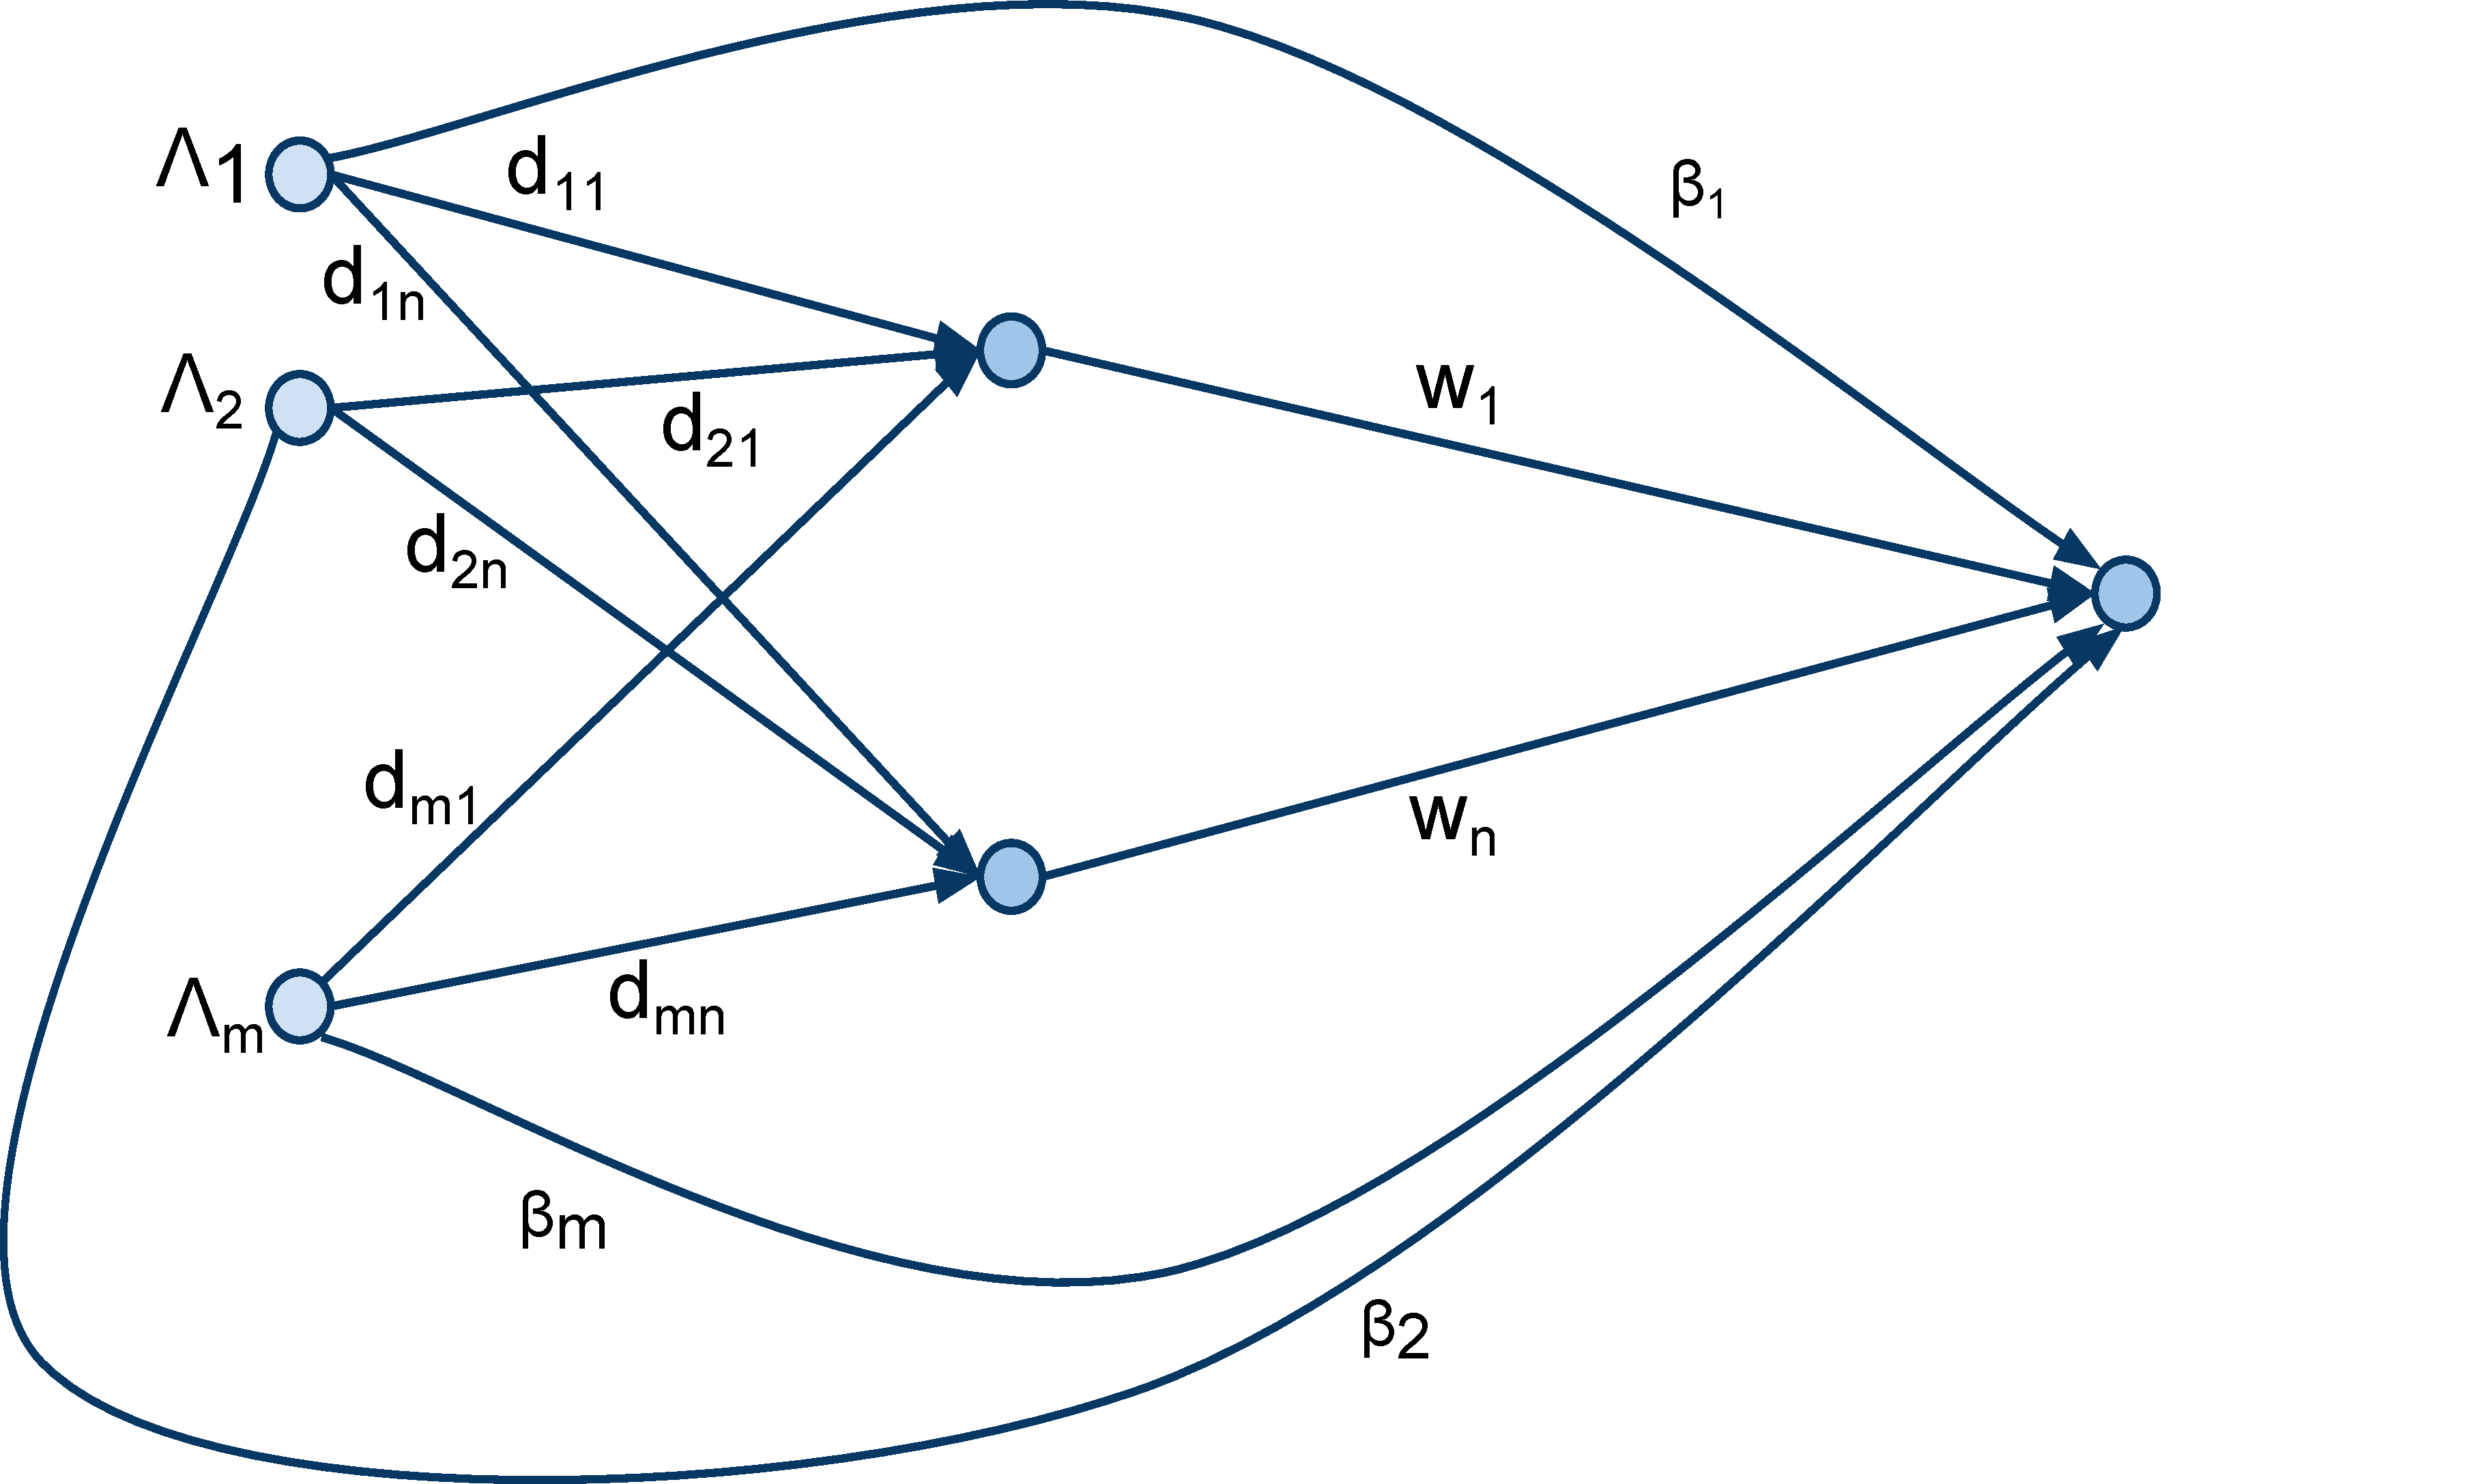
\includegraphics[width=.7\textwidth]{./Images/Hospital_Routing_Game.pdf}
\end{center}
\caption{Routing game: $m$ hospitals to $n$ services.}\label{fig:routinggame}
\end{figure}

The corresponding cost function for a given traffic flow $\lambda$ is given by:

\begin{equation}
C(\lambda)=\sum_{i=1}^m\alpha_i\sum_{j}^nd_{ij}\lambda_{ij}+\sum_{j=1}^n\sum_{i=1}^m\lambda_{ij}w_j\left(\sum_{i=1}^m\lambda_{ij}\right)+\sum_{i=1}^m\beta_i\left(\Lambda_i-\sum_{j=1}^n\lambda_{ij}\right)
\label{C}\end{equation}

The constant $\alpha_i\in\mathbb{R}_{\geq0}$ is simply a weighting statistic for the relative importance of travel distances to the other factors (once again allowing for this coefficient to be dependent on population partitioning).
The Nash flow corresponding to the flow at which all traffic from a given source travels on minimal paths can be shown to be given by the flow that minimises the following function:

\begin{equation}
\Phi(\lambda)=\sum_{i=1}^m\alpha_i\sum_{j}^nd_{ij}\lambda_{ij}+\sum_{j=1}^n\int_0^{\sum_{i=1}^m\lambda_{ij}}w_j(x)dx+\sum_{i=1}^m\beta_i\left(\Lambda_i-\sum_{j=1}^n\lambda_{ij}\right)
\label{Phi}\end{equation}

As a utility function $w_i$ is taken to be the mean waiting time in an $M/M/c$ queue.
From known results on convexity of this measure \cite{lee_note_1983} the following optimisation problems can be solved straightforwardly so as to be able to obtain the PoA for a given instance:

$$\begin{array}{l@{\hspace{2cm}}l}\text{OPTMP:}&\text{NASHMP:}\\
\text{minimise }(\ref{C})&\text{minimise }(\ref{Phi})
\end{array}$$
such that:
\begin{equation}
\sum_{j=1}^n\lambda_{ij}\leq\Lambda_{i}\text{ for all }i\in[m]\label{constraint 1}
\end{equation}
\begin{equation}
\lambda_{ij}\in\mathbb{R}^{m\times n}_{\geq 0}\text{ for all }i\in[m],\;j\in[n]\label{constraint 2}
\end{equation}
\begin{equation}
\sum_{i=1}^m\lambda_{ij}<c_j\mu_j\text{ for all }j\in[n]\label{constraint 3}
\end{equation}

In \cite{Knight2013} various theoretical results are proven with regards to the effect of worth of service on the PoA but also with regards to demand.
The profile of Figure \ref{fig:poaprofile} is shown to hold in general.
A system under very high or very low demand will not suffer greatly from the removal of central control.
Most public service systems are however built to match demand which implies a large PoA.

\begin{figure}[!hbtp]
\begin{center}
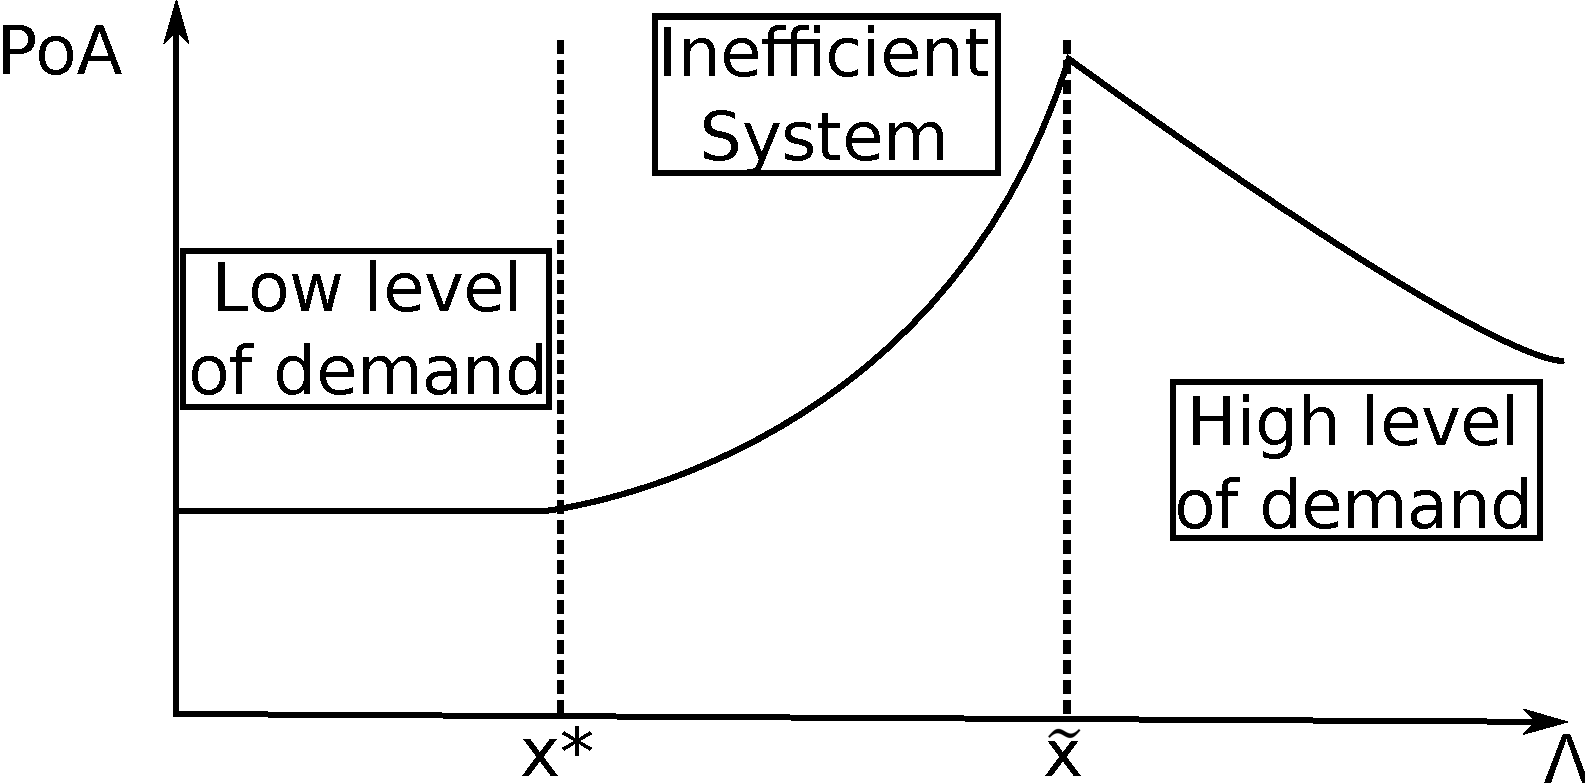
\includegraphics[width=.7\textwidth]{./Images/PoAPlotForSimpleDiagram.pdf}
\end{center}
\caption{General profile of PoA.}\label{fig:poaprofile}
\end{figure}

Further to the theoretical consideration the PoA was calculated for a large case study using Hospital in Wales offering knee surgeries and a high PoA was calculated for the current demand which verifies the previous observation.

To consider systems where individuals are able to observe the system (before making a decision) there are two approaches: the first is to use a simulation based approach that allows individuals to choose their most desirable queue.
One such piece of work that was considered specifically in the context of healthcare is \cite{Knight2010}.

Given that individuals will consider a simple selfish decision rule this approach is relatively straightforward and can also be considered using straightforward analytical Markov models.
The difficulty with this approach appears when attempting to obtain the PoA which requires an optimal routing decision.

In \cite{Shone2014} various dynamic programming and approximate dynamic programming techniques are proposed that are able to not only give an optimal policy but also prove the following observation holds once again:

\begin{center}
\textit{Selfish users make busier systems.}
\end{center}

In the next section selfish congestion related decisions by managers will be considered.

\section{Managing queues}\label{sec:managingqueues}

Following recent analysis of two critical care units (CCUs) it was found that only a state dependent queueing model (where the demand rate to each CCU depended on the state of the CCU) would give a valid representation of the system.
Upon discussion with the CCU managers in question, it was acknowledged that certain behavioural control of admissions occurred, even if it was at a subconscious level.
Indeed when one CCU was at high capacity it was likely to divert patients to the other CCU.

In \cite{knight2014} a normal form game consideration of this situation is given akin to the work on EDs in \cite{Deo2011}.
A pictorial representation of the situation considered is given in Figure \ref{diagramofdiversion} where each CCU can choose a capacity threshold at which to divert patients, and Table \ref{tab:parameters1} shows the parameters used.

\begin{figure}[!htbp]
\begin{center}
\begin{tikzpicture}
\node (A) at (0,0) [draw] {1};
\node (B) at (2,0) [draw] {2};
\draw [->] (-1,0) -- (A);
\draw [->] (3,0) -- (B);
\draw [->] (-1,0) -- ($(A)+(-.5,0)$) -- ($(A)+(-.5,.5)$) -- ($(A)+(.5,.5)$) -- ($(A)+(.5,.1)$) -- ($(B)+(-.4,.1)$);
\draw [->] (3,0) -- ($(B)+(.5,0)$) -- ($(B)+(.5,-.5)$) -- ($(B)+(-.5,-.5)$) -- ($(B)+(-.5,-.1)$) -- ($(A)+(.4,-.1)$);
\draw [->] (3,0) -- (B);
\node at ($(A) + (0,.8)$) {Divert?};
\node at ($(B) + (0,-.8)$) {Divert?};
\end{tikzpicture}
\caption{Diagrammatic representation of CCU interaction through patient diversion.}\label{diagramofdiversion}
\end{center}
\end{figure}


\begin{table}[!hbtp]
\begin{center}
\begin{tabular}{cl}
\toprule
Parameter & Interpretation\\
\midrule
$h\in\{1,2\}$& CCU\\
$c_h$& Capacity of CCU\\
$K_h$& Cutoff strategy of CCU\\
$\lambda_{h}^{\text{area}}$& Demand rate as described in Figure \ref{arrivalrateregions}\\
$\mu_{h}$&Service rate of CCU\\
\toprule
\end{tabular}
\caption{Parameters of CCU model}\label{tab:parameters1}
\end{center}
\end{table}

The capacity thresholds are denoted as $K_{h}\in\mathbb{Z}$ for $h\in\{1,2\}$, once diverted the arrival rate is modified as shown in Figure \ref{arrivalrateregions}.
In general it is assumed that $\lambda_h^{(a)}\geq \lambda_{h}^{(b)}, \lambda_{h}^{(c)}\geq \lambda_{h}^{(d)}$ (so that setting a diversion threshold implies a reduction of patient flow).
Note that $0\leq K_h\leq c_h$.

\begin{figure}[!htbp]
\begin{center}
    \begin{tikzpicture}
        \draw  (0,0) rectangle (4,3);
        \draw [dashed, red, thick] (0,1) -- (4,1);
        \draw [dashed, red, thick] (3,0) -- (3,3);
        \node at (-.5,1) {$K_{1}$};
        \node at (3,3.25) {$K_{2}$};
        \node at (1.5,2) {$\lambda_{h}^{(a)}$};
        \node at (3.5,2) {$\lambda_{h}^{(b)}$};
        \node at (1.5,.5) {$\lambda_{h}^{(c)}$};
        \node at (3.5,.5) {$\lambda_{h}^{(d)}$};
    \end{tikzpicture}
\caption{General arrival rates for each CCU at each region, where $h\in\{1, 2\}$} \label{arrivalrateregions}
\end{center}
\end{figure}

\begin{figure}[!htbp]
\begin{center}
\begin{tikzpicture}[scale=.7, every node/.style={scale=0.7}]
    % -----------------------------------------------
    % Boundaries ------------------------------------
    % -----------------------------------------------
    \draw [dashed, line width=1mm, red, opacity=.3] (12,2) -- (12,-20);
    \draw [dashed, line width=1mm, red, opacity=.3] (-2,-12) -- (20,-12);
    %\tikzstyle{state}=[ellipse, draw, fill=blue!10, minimum width=2cm];
    %\tikzstyle{state}=[rectangle, draw, fill=blue!10, minimum width=2cm];
    \tikzstyle{state}=[minimum width=2cm, font=\boldmath];
    %\draw  (0,0) rectangle (4,3);
    %\draw [dashed, red, thick] (0,1) -- (4,1);
    %\draw [dashed, red, thick] (3,0) -- (3,3);
    % -----------------------------------------------
    % First row--------------------------------------
    % -----------------------------------------------
    \node (aa) [state] at (0,0) {$(0,0)$};
    \node (ab) [state] at ($(aa) + (3,0)$) {$(0,1)$};
    \node (ac) [state] at ($(ab) + (3,0)$) {$(0,2)$};
    \node (ellipsisa1) at ($(ac) + (3,0)$) {$\dots$};
    \node(ak) [state] at ($(ellipsisa1) + (3,0)$) {$(0,K_{1})$};
    \node (ellipsisa2) at ($(ak) + (3,0)$) {$\dots$};
    \node(az) [state] at ($(ellipsisa2) + (3,0)$) {$(0,c_{1})$};
    % Transitions -----------------------------------
    % On Row:
    \draw (aa) edge[out=45,in=135,->,thick] node [above] {\tiny$\lambda_{1}^{(a)}$} (ab);
    \draw (aa) edge[out=-45,in=-135,<-,thick] node [below] {\tiny$\mu_{1}$} (ab);

    \draw (ab) edge[out=45,in=135,->,thick] node [above] {\tiny$\lambda_{1}^{(a)}$} (ac);
    \draw (ab) edge[out=-45,in=-135,<-,thick] node [below] {\tiny$\mu_{1}$} (ac);

    \draw (ac) edge[out=45,in=135,->,thick] node [above] {\tiny$\lambda_{1}^{(a)}$} (ellipsisa1);
    \draw (ac) edge[out=-45,in=-135,<-,thick] node [below] {\tiny$\mu_{1}$} (ellipsisa1);

    \draw (ellipsisa1) edge[out=45,in=135,->,thick] node [above] {\tiny$\lambda_{1}^{(a)}$} (ak);
    \draw (ellipsisa1) edge[out=-45,in=-135,<-,thick] node [below] {\tiny$\mu_{1}$} (ak);

    \draw (ak) edge[out=45,in=135,->,thick] node [above] {\tiny$\lambda_{1}^{(b)}$} (ellipsisa2);
    \draw (ak) edge[out=-45,in=-135,<-,thick] node [below] {\tiny$\mu_{1}$} (ellipsisa2);

    \draw (ellipsisa2) edge[out=45,in=135,->,thick] node [above] {\tiny$\lambda_{1}^{(b)}$} (az);
    \draw (ellipsisa2) edge[out=-45,in=-135,<-,thick] node [below] {\tiny$\mu_{1}$} (az);
    % -----------------------------------------------
    % Second row--------------------------------------
    % -----------------------------------------------
    \node (ba) [state] at (0,-3) {$(1,0)$};
    \node (bb) [state] at ($(ba) + (3,0)$) {$(1,1)$};
    \node (bc) [state] at ($(bb) + (3,0)$) {$(1,2)$};
    \node (ellipsisb1) at ($(bc) + (3,0)$) {$\dots$};
    \node(bk) [state] at ($(ellipsisb1) + (3,0)$) {$(1,K_{1})$};
    \node (ellipsisb2) at ($(bk) + (3,0)$) {$\dots$};
    \node(bz) [state] at ($(ellipsisb2) + (3,0)$) {$(1,c_{1})$};
    % Transitions -----------------------------------
    % On Row:
    \draw (ba) edge[out=45,in=135,->,thick] node [above] {\tiny$\lambda_{1}^{(a)}$} (bb);
    \draw (ba) edge[out=-45,in=-135,<-,thick] node [below] {\tiny$\mu_{1}$} (bb);

    \draw (bb) edge[out=45,in=135,->,thick] node [above] {\tiny$\lambda_{1}^{(a)}$} (bc);
    \draw (bb) edge[out=-45,in=-135,<-,thick] node [below] {\tiny$\mu_{1}$} (bc);

    \draw (bc) edge[out=45,in=135,->,thick] node [above] {\tiny$\lambda_{1}^{(a)}$} (ellipsisb1);
    \draw (bc) edge[out=-45,in=-135,<-,thick] node [below] {\tiny$\mu_{1}$} (ellipsisb1);

    \draw (ellipsisb1) edge[out=45,in=135,->,thick] node [above] {\tiny$\lambda_{1}^{(a)}$} (bk);
    \draw (ellipsisb1) edge[out=-45,in=-135,<-,thick] node [below] {\tiny$\mu_{1}$} (bk);

    \draw (bk) edge[out=45,in=135,->,thick] node [above] {\tiny$\lambda_{1}^{(b)}$} (ellipsisb2);
    \draw (bk) edge[out=-45,in=-135,<-,thick] node [below] {\tiny$\mu_{1}$} (ellipsisb2);

    \draw (ellipsisb2) edge[out=45,in=135,->,thick] node [above] {\tiny$\lambda_{1}^{(b)}$} (bz);
    \draw (ellipsisb2) edge[out=-45,in=-135,<-,thick] node [below] {\tiny$\mu_{1}$} (bz);
    % With previous row:
    \draw (aa) edge[out=-125,in=125,->,thick] node [left] {\tiny$\lambda_{2}^{(a)}$} (ba);
    \draw (aa) edge[out=-55,in=55,<-,thick] node [right] {\tiny$\mu_{2}$} (ba);

    \draw (ab) edge[out=-125,in=125,->,thick] node [left] {\tiny$\lambda_{2}^{(a)}$} (bb);
    \draw (ab) edge[out=-55,in=55,<-,thick] node [right] {\tiny$\mu_{2}$} (bb);

    \draw (ac) edge[out=-125,in=125,->,thick] node [left] {\tiny$\lambda_{2}^{(a)}$} (bc);
    \draw (ac) edge[out=-55,in=55,<-,thick] node [right] {\tiny$\mu_{2}$} (bc);

    \draw (ellipsisa1) edge[out=-125,in=125,->,thick] node [left] {\tiny$\lambda_{2}^{(a)}$} (ellipsisb1);
    \draw (ellipsisa1) edge[out=-55,in=55,<-,thick] node [right] {\tiny$\mu_{2}$} (ellipsisb1);

    \draw (ak) edge[out=-125,in=125,->,thick] node [left] {\tiny$\lambda_{2}^{(b)}$} (bk);
    \draw (ak) edge[out=-55,in=55,<-,thick] node [right] {\tiny$\mu_{2}$} (bk);

    \draw (ellipsisa2) edge[out=-125,in=125,->,thick] node [left] {\tiny$\lambda_{2}^{(b)}$} (ellipsisb2);
    \draw (ellipsisa2) edge[out=-55,in=55,<-,thick] node [right] {\tiny$\mu_{2}$} (ellipsisb2);

    \draw (az) edge[out=-125,in=125,->,thick] node [left] {\tiny$\lambda_{2}^{(b)}$} (bz);
    \draw (az) edge[out=-55,in=55,<-,thick] node [right] {\tiny$\mu_{2}$} (bz);
    % -----------------------------------------------
    % Third row--------------------------------------
    % -----------------------------------------------
    \node (ca) [state] at (0,-6) {$(2,0)$};
    \node (cb) [state] at ($(ca) + (3,0)$) {$(2,1)$};
    \node (cc) [state] at ($(cb) + (3,0)$) {$(2,2)$};
    \node (ellipsisc1) at ($(cc) + (3,0)$) {$\dots$};
    \node(ck) [state] at ($(ellipsisc1) + (3,0)$) {$(2,K_{1})$};
    \node (ellipsisc2) at ($(ck) + (3,0)$) {$\dots$};
    \node(cz) [state] at ($(ellipsisc2) + (3,0)$) {$(2,c_{1})$};
    % Transitions -----------------------------------
    % On Row:
    \draw (ca) edge[out=45,in=135,->,thick] node [above] {\tiny$\lambda_{1}^{(a)}$} (cb);
    \draw (ca) edge[out=-45,in=-135,<-,thick] node [below] {\tiny$\mu_{1}$} (cb);

    \draw (cb) edge[out=45,in=135,->,thick] node [above] {\tiny$\lambda_{1}^{(a)}$} (cc);
    \draw (cb) edge[out=-45,in=-135,<-,thick] node [below] {\tiny$\mu_{1}$} (cc);

    \draw (cc) edge[out=45,in=135,->,thick] node [above] {\tiny$\lambda_{1}^{(a)}$} (ellipsisc1);
    \draw (cc) edge[out=-45,in=-135,<-,thick] node [below] {\tiny$\mu_{1}$} (ellipsisc1);

    \draw (ellipsisc1) edge[out=45,in=135,->,thick] node [above] {\tiny$\lambda_{1}^{(a)}$} (ck);
    \draw (ellipsisc1) edge[out=-45,in=-135,<-,thick] node [below] {\tiny$\mu_{1}$} (ck);

    \draw (ck) edge[out=45,in=135,->,thick] node [above] {\tiny$\lambda_{1}^{(b)}$} (ellipsisc2);
    \draw (ck) edge[out=-45,in=-135,<-,thick] node [below] {\tiny$\mu_{1}$} (ellipsisc2);

    \draw (ellipsisc2) edge[out=45,in=135,->,thick] node [above] {\tiny$\lambda_{1}^{(b)}$} (cz);
    \draw (ellipsisc2) edge[out=-45,in=-135,<-,thick] node [below] {\tiny$\mu_{1}$} (cz);
    % With previous row:
    \draw (ba) edge[out=-125,in=125,->,thick] node [left] {\tiny$\lambda_{2}^{(a)}$} (ca);
    \draw (ba) edge[out=-55,in=55,<-,thick] node [right] {\tiny$\mu_{2}$} (ca);

    \draw (bb) edge[out=-125,in=125,->,thick] node [left] {\tiny$\lambda_{2}^{(a)}$} (cb);
    \draw (bb) edge[out=-55,in=55,<-,thick] node [right] {\tiny$\mu_{2}$} (cb);

    \draw (bc) edge[out=-125,in=125,->,thick] node [left] {\tiny$\lambda_{2}^{(a)}$} (cc);
    \draw (bc) edge[out=-55,in=55,<-,thick] node [right] {\tiny$\mu_{2}$} (cc);

    \draw (ellipsisb1) edge[out=-125,in=125,->,thick] node [left] {\tiny$\lambda_{2}^{(a)}$} (ellipsisc1);
    \draw (ellipsisb1) edge[out=-55,in=55,<-,thick] node [right] {\tiny$\mu_{2}$} (ellipsisc1);

    \draw (bk) edge[out=-125,in=125,->,thick] node [left] {\tiny$\lambda_{2}^{(b)}$} (ck);
    \draw (bk) edge[out=-55,in=55,<-,thick] node [right] {\tiny$\mu_{2}$} (ck);

    \draw (ellipsisb2) edge[out=-125,in=125,->,thick] node [left] {\tiny$\lambda_{2}^{(b)}$} (ellipsisc2);
    \draw (ellipsisb2) edge[out=-55,in=55,<-,thick] node [right] {\tiny$\mu_{2}$} (ellipsisc2);

    \draw (bz) edge[out=-125,in=125,->,thick] node [left] {\tiny$\lambda_{2}^{(b)}$} (cz);
    \draw (bz) edge[out=-55,in=55,<-,thick] node [right] {\tiny$\mu_{2}$} (cz);
    % -----------------------------------------------
    % Fourth row--------------------------------------
    % -----------------------------------------------
    \node (da) at (0,-9) {$\vdots$};
    \node (db) at ($(da) + (3,0)$) {$\vdots$};
    \node (dc) at ($(db) + (3,0)$) {$\vdots$};
    \node (ellipsisd1) at ($(dc) + (3,0)$) {$\dots$};
    \node(dk) at ($(ellipsisd1) + (3,0)$) {$\vdots$};
    \node (ellipsisd2) at ($(dk) + (3,0)$) {$\dots$};
    \node(dz) at ($(ellipsisd2) + (3,0)$) {$\vdots$};
    % Transitions -----------------------------------
    % On Row:
    \draw (da) edge[out=45,in=135,->,thick] node [above] {\tiny$\lambda_{1}^{(a)}$} (db);
    \draw (da) edge[out=-45,in=-135,<-,thick] node [below] {\tiny$\mu_{1}$} (db);

    \draw (db) edge[out=45,in=135,->,thick] node [above] {\tiny$\lambda_{1}^{(a)}$} (dc);
    \draw (db) edge[out=-45,in=-135,<-,thick] node [below] {\tiny$\mu_{1}$} (dc);

    \draw (dc) edge[out=45,in=135,->,thick] node [above] {\tiny$\lambda_{1}^{(a)}$} (ellipsisd1);
    \draw (dc) edge[out=-45,in=-135,<-,thick] node [below] {\tiny$\mu_{1}$} (ellipsisd1);

    \draw (ellipsisd1) edge[out=45,in=135,->,thick] node [above] {\tiny$\lambda_{1}^{(a)}$} (dk);
    \draw (ellipsisd1) edge[out=-45,in=-135,<-,thick] node [below] {\tiny$\mu_{1}$} (dk);

    \draw (dk) edge[out=45,in=135,->,thick] node [above] {\tiny$\lambda_{1}^{(b)}$} (ellipsisd2);
    \draw (dk) edge[out=-45,in=-135,<-,thick] node [below] {\tiny$\mu_{1}$} (ellipsisd2);

    \draw (ellipsisd2) edge[out=45,in=135,->,thick] node [above] {\tiny$\lambda_{1}^{(b)}$} (dz);
    \draw (ellipsisd2) edge[out=-45,in=-135,<-,thick] node [below] {\tiny$\mu_{1}$} (dz);
    % With previous row:
    \draw (ca) edge[out=-125,in=125,->,thick] node [left] {\tiny$\lambda_{2}^{(a)}$} (da);
    \draw (ca) edge[out=-55,in=55,<-,thick] node [right] {\tiny$\mu_{2}$} (da);

    \draw (cb) edge[out=-125,in=125,->,thick] node [left] {\tiny$\lambda_{2}^{(a)}$} (db);
    \draw (cb) edge[out=-55,in=55,<-,thick] node [right] {\tiny$\mu_{2}$} (db);

    \draw (cc) edge[out=-125,in=125,->,thick] node [left] {\tiny$\lambda_{2}^{(a)}$} (dc);
    \draw (cc) edge[out=-55,in=55,<-,thick] node [right] {\tiny$\mu_{2}$} (dc);

    \draw (ellipsisc1) edge[out=-125,in=125,->,thick] node [left] {\tiny$\lambda_{2}^{(a)}$} (ellipsisd1);
    \draw (ellipsisc1) edge[out=-55,in=55,<-,thick] node [right] {\tiny$\mu_{2}$} (ellipsisd1);

    \draw (ck) edge[out=-125,in=125,->,thick] node [left] {\tiny$\lambda_{2}^{(b)}$} (dk);
    \draw (ck) edge[out=-55,in=55,<-,thick] node [right] {\tiny$\mu_{2}$} (dk);

    \draw (ellipsisc2) edge[out=-125,in=125,->,thick] node [left] {\tiny$\lambda_{2}^{(b)}$} (ellipsisd2);
    \draw (ellipsisc2) edge[out=-55,in=55,<-,thick] node [right] {\tiny$\mu_{2}$} (ellipsisd2);

    \draw (cz) edge[out=-125,in=125,->,thick] node [left] {\tiny$\lambda_{2}^{(b)}$} (dz);
    \draw (cz) edge[out=-55,in=55,<-,thick] node [right] {\tiny$\mu_{2}$} (dz);
    % -----------------------------------------------
    % Fifth row--------------------------------------
    % -----------------------------------------------
    \node (ea) [state] at (0,-12) {$(K_{2},0)$};
    \node (eb) [state] at ($(ea) + (3,0)$) {$(K_{2},1)$};
    \node (ec) [state] at ($(eb) + (3,0)$) {$(K_{2},2)$};
    \node (ellipsise1) at ($(ec) + (3,0)$) {$\dots$};
    \node(ek) [state] at ($(ellipsise1) + (3,0)$) {$(K_{2},K_{1})$};
    \node (ellipsise2) at ($(ek) + (3,0)$) {$\dots$};
    \node(ez) [state] at ($(ellipsise2) + (3,0)$) {$(K_{2},c_{1})$};
    % Transitions -----------------------------------
    % On Row:
    \draw (ea) edge[out=45,in=135,->,thick] node [above] {\tiny$\lambda_{1}^{(c)}$} (eb);
    \draw (ea) edge[out=-45,in=-135,<-,thick] node [below] {\tiny$\mu_{1}$} (eb);

    \draw (eb) edge[out=45,in=135,->,thick] node [above] {\tiny$\lambda_{1}^{(c)}$} (ec);
    \draw (eb) edge[out=-45,in=-135,<-,thick] node [below] {\tiny$\mu_{1}$} (ec);

    \draw (ec) edge[out=45,in=135,->,thick] node [above] {\tiny$\lambda_{1}^{(c)}$} (ellipsise1);
    \draw (ec) edge[out=-45,in=-135,<-,thick] node [below] {\tiny$\mu_{1}$} (ellipsise1);

    \draw (ellipsise1) edge[out=45,in=135,->,thick] node [above] {\tiny$\lambda_{1}^{(c)}$} (ek);
    \draw (ellipsise1) edge[out=-45,in=-135,<-,thick] node [below] {\tiny$\mu_{1}$} (ek);

    \draw (ek) edge[out=45,in=135,->,thick] node [above] {\tiny$\lambda_{1}^{(d)}$} (ellipsise2);
    \draw (ek) edge[out=-45,in=-135,<-,thick] node [below] {\tiny$\mu_{1}$} (ellipsise2);

    \draw (ellipsise2) edge[out=45,in=135,->,thick] node [above] {\tiny$\lambda_{1}^{(d)}$} (ez);
    \draw (ellipsise2) edge[out=-45,in=-135,<-,thick] node [below] {\tiny$\mu_{1}$} (ez);
    % With previous row:
    \draw (da) edge[out=-125,in=125,->,thick] node [left] {\tiny$\lambda_{2}^{(a)}$} (ea);
    \draw (da) edge[out=-55,in=55,<-,thick] node [right] {\tiny$\mu_{2}$} (ea);

    \draw (db) edge[out=-125,in=125,->,thick] node [left] {\tiny$\lambda_{2}^{(a)}$} (eb);
    \draw (db) edge[out=-55,in=55,<-,thick] node [right] {\tiny$\mu_{2}$} (eb);

    \draw (dc) edge[out=-125,in=125,->,thick] node [left] {\tiny$\lambda_{2}^{(a)}$} (ec);
    \draw (dc) edge[out=-55,in=55,<-,thick] node [right] {\tiny$\mu_{2}$} (ec);

    \draw (ellipsisd1) edge[out=-125,in=125,->,thick] node [left] {\tiny$\lambda_{2}^{(a)}$} (ellipsise1);
    \draw (ellipsisd1) edge[out=-55,in=55,<-,thick] node [right] {\tiny$\mu_{2}$} (ellipsise1);

    \draw (dk) edge[out=-125,in=125,->,thick] node [left] {\tiny$\lambda_{2}^{(b)}$} (ek);
    \draw (dk) edge[out=-55,in=55,<-,thick] node [right] {\tiny$\mu_{2}$} (ek);

    \draw (ellipsisd2) edge[out=-125,in=125,->,thick] node [left] {\tiny$\lambda_{2}^{(b)}$} (ellipsise2);
    \draw (ellipsisd2) edge[out=-55,in=55,<-,thick] node [right] {\tiny$\mu_{2}$} (ellipsise2);

    \draw (dz) edge[out=-125,in=125,->,thick] node [left] {\tiny$\lambda_{2}^{(b)}$} (ez);
    \draw (dz) edge[out=-55,in=55,<-,thick] node [right] {\tiny$\mu_{2}$} (ez);
    % Sixth row--------------------------------------
    \node (fa) at (0,-15) {$\vdots$};
    \node (fb) at ($(fa) + (3,0)$) {$\vdots$};
    \node (fc) at ($(fb) + (3,0)$) {$\vdots$};
    \node (ellipsisf1) at ($(fc) + (3,0)$) {$\dots$};
    \node(fk) at ($(ellipsisf1) + (3,0)$) {$\vdots$};
    \node (ellipsisf2) at ($(fk) + (3,0)$) {$\dots$};
    \node(fz) at ($(ellipsisf2) + (3,0)$) {$\vdots$};
    % Transitions -----------------------------------
    % On Row:
    \draw (fa) edge[out=45,in=135,->,thick] node [above] {\tiny$\lambda_{1}^{(c)}$} (fb);
    \draw (fa) edge[out=-45,in=-135,<-,thick] node [below] {\tiny$\mu_{1}$} (fb);

    \draw (fb) edge[out=45,in=135,->,thick] node [above] {\tiny$\lambda_{1}^{(c)}$} (fc);
    \draw (fb) edge[out=-45,in=-135,<-,thick] node [below] {\tiny$\mu_{1}$} (fc);

    \draw (fc) edge[out=45,in=135,->,thick] node [above] {\tiny$\lambda_{1}^{(c)}$} (ellipsisf1);
    \draw (fc) edge[out=-45,in=-135,<-,thick] node [below] {\tiny$\mu_{1}$} (ellipsisf1);

    \draw (ellipsisf1) edge[out=45,in=135,->,thick] node [above] {\tiny$\lambda_{1}^{(c)}$} (fk);
    \draw (ellipsisf1) edge[out=-45,in=-135,<-,thick] node [below] {\tiny$\mu_{1}$} (fk);

    \draw (fk) edge[out=45,in=135,->,thick] node [above] {\tiny$\lambda_{1}^{(d)}$} (ellipsisf2);
    \draw (fk) edge[out=-45,in=-135,<-,thick] node [below] {\tiny$\mu_{1}$} (ellipsisf2);

    \draw (ellipsisf2) edge[out=45,in=135,->,thick] node [above] {\tiny$\lambda_{1}^{(d)}$} (fz);
    \draw (ellipsisf2) edge[out=-45,in=-135,<-,thick] node [below] {\tiny$\mu_{1}$} (fz);
    % With previous row:
    \draw (ea) edge[out=-125,in=125,->,thick] node [left] {\tiny$\lambda_{2}^{(c)}$} (fa);
    \draw (ea) edge[out=-55,in=55,<-,thick] node [right] {\tiny$\mu_{2}$} (fa);

    \draw (eb) edge[out=-125,in=125,->,thick] node [left] {\tiny$\lambda_{2}^{(c)}$} (fb);
    \draw (eb) edge[out=-55,in=55,<-,thick] node [right] {\tiny$\mu_{2}$} (fb);

    \draw (ec) edge[out=-125,in=125,->,thick] node [left] {\tiny$\lambda_{2}^{(c)}$} (fc);
    \draw (ec) edge[out=-55,in=55,<-,thick] node [right] {\tiny$\mu_{2}$} (fc);

    \draw (ellipsise1) edge[out=-125,in=125,->,thick] node [left] {\tiny$\lambda_{2}^{(c)}$} (ellipsisf1);
    \draw (ellipsise1) edge[out=-55,in=55,<-,thick] node [right] {\tiny$\mu_{2}$} (ellipsisf1);

    \draw (ek) edge[out=-125,in=125,->,thick] node [left] {\tiny$\lambda_{2}^{(d)}$} (fk);
    \draw (ek) edge[out=-55,in=55,<-,thick] node [right] {\tiny$\mu_{2}$} (fk);

    \draw (ellipsise2) edge[out=-125,in=125,->,thick] node [left] {\tiny$\lambda_{2}^{(d)}$} (ellipsisf2);
    \draw (ellipsise2) edge[out=-55,in=55,<-,thick] node [right] {\tiny$\mu_{2}$} (ellipsisf2);

    \draw (ez) edge[out=-125,in=125,->,thick] node [left] {\tiny$\lambda_{2}^{(d)}$} (fz);
    \draw (ez) edge[out=-55,in=55,<-,thick] node [right] {\tiny$\mu_{2}$} (fz);
    % Final row--------------------------------------
    \node (za) [state] at (0,-18) {$(c_{2},0)$};
    \node (zb) [state] at ($(za) + (3,0)$) {$(c_{2},1)$};
    \node (zc) [state] at ($(zb) + (3,0)$) {$(c_{2},2)$};
    \node (ellipsisz1) at ($(zc) + (3,0)$) {$\dots$};
    \node(zk) [state] at ($(ellipsisz1) + (3,0)$) {$(c_{2},K_{1})$};
    \node (ellipsisz2) at ($(zk) + (3,0)$) {$\dots$};
    \node(zz) [state] at ($(ellipsisz2) + (3,0)$) {$(c_{2},c_{1})$};
    % Transitions -----------------------------------
    % On Row:
    \draw (za) edge[out=45,in=135,->,thick] node [above] {\tiny$\lambda_{1}^{(d)}$} (zb);
    \draw (za) edge[out=-45,in=-135,<-,thick] node [below] {\tiny$\mu_{1}$} (zb);

    \draw (zb) edge[out=45,in=135,->,thick] node [above] {\tiny$\lambda_{1}^{(d)}$} (zc);
    \draw (zb) edge[out=-45,in=-135,<-,thick] node [below] {\tiny$\mu_{1}$} (zc);

    \draw (zc) edge[out=45,in=135,->,thick] node [above] {\tiny$\lambda_{1}^{(d)}$} (ellipsisz1);
    \draw (zc) edge[out=-45,in=-135,<-,thick] node [below] {\tiny$\mu_{1}$} (ellipsisz1);

    \draw (ellipsisz1) edge[out=45,in=135,->,thick] node [above] {\tiny$\lambda_{1}^{(d)}$} (zk);
    \draw (ellipsisz1) edge[out=-45,in=-135,<-,thick] node [below] {\tiny$\mu_{1}$} (zk);

    \draw (zk) edge[out=45,in=135,->,thick] node [above] {\tiny$\lambda_{1}^{(d)}$} (ellipsisz2);
    \draw (zk) edge[out=-45,in=-135,<-,thick] node [below] {\tiny$\mu_{1}$} (ellipsisz2);

    \draw (ellipsisz2) edge[out=45,in=135,->,thick] node [above] {\tiny$\lambda_{1}^{(d)}$} (zz);
    \draw (ellipsisz2) edge[out=-45,in=-135,<-,thick] node [below] {\tiny$\mu_{1}$} (zz);
    % With previous row:
    \draw (fa) edge[out=-125,in=125,->,thick] node [left] {\tiny$\lambda_{2}^{(c)}$} (za);
    \draw (fa) edge[out=-55,in=55,<-,thick] node [right] {\tiny$\mu_{2}$} (za);

    \draw (fb) edge[out=-125,in=125,->,thick] node [left] {\tiny$\lambda_{2}^{(c)}$} (zb);
    \draw (fb) edge[out=-55,in=55,<-,thick] node [right] {\tiny$\mu_{2}$} (zb);

    \draw (fc) edge[out=-125,in=125,->,thick] node [left] {\tiny$\lambda_{2}^{(c)}$} (zc);
    \draw (fc) edge[out=-55,in=55,<-,thick] node [right] {\tiny$\mu_{2}$} (zc);

    \draw (ellipsisf1) edge[out=-125,in=125,->,thick] node [left] {\tiny$\lambda_{2}^{(c)}$} (ellipsisz1);
    \draw (ellipsisf1) edge[out=-55,in=55,<-,thick] node [right] {\tiny$\mu_{2}$} (ellipsisz1);

    \draw (fk) edge[out=-125,in=125,->,thick] node [left] {\tiny$\lambda_{2}^{(d)}$} (zk);
    \draw (fk) edge[out=-55,in=55,<-,thick] node [right] {\tiny$\mu_{2}$} (zk);

    \draw (ellipsisf2) edge[out=-125,in=125,->,thick] node [left] {\tiny$\lambda_{2}^{(d)}$} (ellipsisz2);
    \draw (ellipsisf2) edge[out=-55,in=55,<-,thick] node [right] {\tiny$\mu_{2}$} (ellipsisz2);

    \draw (fz) edge[out=-125,in=125,->,thick] node [left] {\tiny$\lambda_{2}^{(d)}$} (zz);
    \draw (fz) edge[out=-55,in=55,<-,thick] node [right] {\tiny$\mu_{2}$} (zz);

\end{tikzpicture}

\caption{Generic Markov chain underpinning the queueing model of this paper} \label{mc}
\end{center}
\end{figure}

Throughput of patients is a natural choice of utility for the game theoretic model given that most hospitals are financially rewarded per served patient \cite{Pate2009}.
For each threshold pair $(K_{1},K_{2})$, the utilisation rate $U_h$ and throughput $T_h$ can easily be obtained for each CCU: $h\in\{\text{1},\text{2}\}$, using the following formulas:

$$U_{h}={{\sum_{n=0}^{c_h} nP^{(h)}(n)}\over{c_{h}}}$$
$$T_{h}=\mu_h \sum _{n=0}^{c_h} nP^{(h)}(n)$$

where $P^{(h)}=P^{(h)}(K_{1},K_{2})$ is the steady state probability distribution function (obtained from by analysing the Markov chain of Figure \ref{mc}).

The optimisation problem faced by each hospital that gives rise to the game is:

For all $h\in\{\text{1}, \text{2}\}$ minimise:
\begin{equation}\left(U_{h}-t\right)^2\end{equation}
Subject to:
\begin{equation}
0\leq K_h \leq c_{h}
\end{equation}
\begin{equation}
K_h \in  \mathbb{Z}
\end{equation}

This game is equivalent to a bi matrix game with restriction to pure strategies where both players aim to get their utilisation as close as possible to a certain target.
As such a Nash Equilibrium is not guaranteed by traditional game theoretical results \cite{Nash1950}, but based on discussions with ABUHB, long term threshold policies are a realistic consideration.
In \cite{knight2014} theoretical results are proved that guarentee pure strategy Nash equilibria in certain cases.

Using this and structural properties of the problem a Nash equilibria can be found.
A variety of numerical results are shown giving the PoA for various scenarios but importantly this module can aid in the informed assignment of a policy $t$.
Figure \ref{mintargetvdemandmodel2} show the smallest value of $t$ that gives a PoA for a variation of demand ($x=0$ corresponds to the actual demand of the system in consideration).
This value was obtained in a model where CCUs could divert demand unless both CCUs are in diversion in which case CCUs must deal with their own demand.

\begin{figure}[!htbp]
\begin{center}
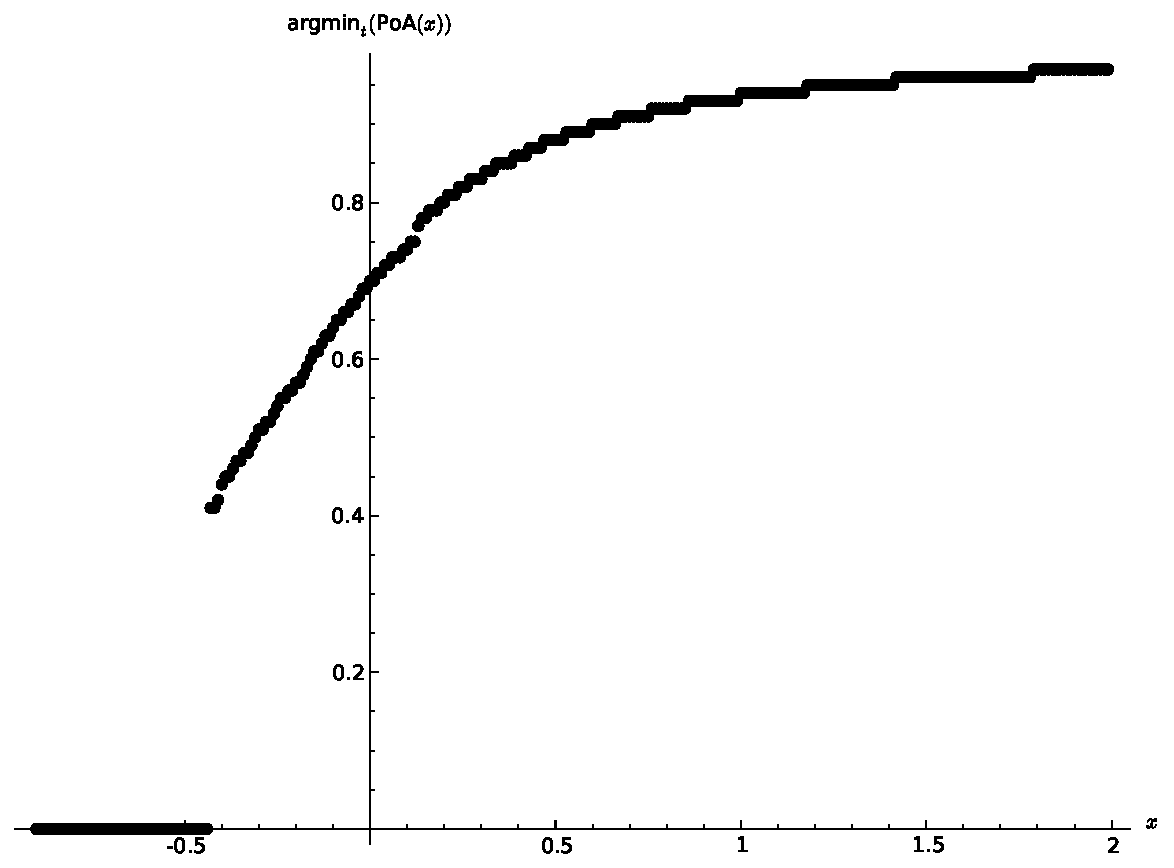
\includegraphics[width=12cm]{./Images/argminPoAmodel2.pdf}
\caption{Lowest value of $t$ ensuring PoA$=1$} \label{mintargetvdemandmodel2}
\end{center}
\end{figure}

We see that a value of $t=.72$ is recommended for the actual demand of the system.
While this value does not necessarily give an exact value worth installing as policy the methodology gives a valid approach to indicating a sensible target.
Furthermore, as demand increases, we see that the recommended target value increases so as to align the goals of the facilities align with the goals of the overall system.

\section{Conclusions}\label{sec:conclusion}

In this manuscript two game theoretic models applied to healthcare have been considered:

\begin{itemize}
    \item Modelling choices of patients;
    \item Modelling choices of managers.
\end{itemize}

The effect of stochasticity in healthcare systems is well understood and there is a wealth of research to match this.
The effect of individual behaviour is less understood.
Game theory and Price of Anarchy analysis offers one way to measure this effect.

Importantly, there are a variety of further avenues for this exciting area of research:

\begin{itemize}
    \item Games involving players from different parts of a hospital and/or multiple hospitals;
    \item Machine loading games which can be applied to scheduling tasks;
    \item Further policy informing work.
\end{itemize}

With regards to methodological approaches there are a variety of tools available.
Firstly, one can model particular systems with parameters corresponding to the strategies of players (similar to the work described in Section \ref{sec:managingqueues}).
Secondly, there are specific game theoretic models that can be applied directly to healthcare systems (similar to the work described in Section \ref{sec:choosingqueues}).
Finally there are also a variety of novel approaches that can be used such as using evolutionary game theoretic models.
Specific heuristic approaches relevant to Markov Decision Process in both optimal and selfish calculations offer interesting avenues for research.

The fact that optimal behaviour and selfish behaviour are two sides of the same coin is well understood in unobservable queues.
Finding similar connections in observable queues is an open research problem.

\newpage
\bibliographystyle{plain}
\bibliography{library}

%\bigskip
%\noindent{\bf Refer\^encias}
%
%\noindent \textbf {Anna, A.} (1996), Comunica\c c\~ao, \textit{Atas do XXVIII SBPO}, 123-134.
%
%\noindent \textbf{Gates, B.}, \textit{Um Livro Muito Bom}, Editor, Local, 2003.
%
%\noindent  \textbf{Pel\'e, E. N. e Rom\'ario, R. R.}, Exemplo de artigo em livro, em Windows, P. T. e Linux, V. G. (Eds.),
%\textit{Colet\^ania de Artigos},  Editor, Local, 123-133, 2004.
%
%\noindent  \textbf{Silva, A. B., Souza, C. D. e Santos, E. F.}, T\'\i tulo de um relat\'orio t\'ecnico dispon\'\i vel na Internet,
%\textit{ Relat\'orios de Pesquisa em Engenharia de Produ\c c\~ao}, n. 4,  Universidade Z,
%1999
%
%\noindent{(www.universidade.br/rel, 4, 2001.}
%
%\noindent  \textbf{Smith, S. e Jones, J.} (2002), A paper on Operations Research, \textit{Pesquisa Operacional},
%32, 5-44.

\end{document}
